\documentclass[10pt]{beamer}

\usepackage[utf8]{inputenc}
\usepackage[francais]{babel}
\usepackage[T1]{fontenc}
\usepackage{amsmath}
\usepackage{eufrak}
\usepackage{tikz}
\usepackage{graphicx}
\usepackage{textcomp}
\usepackage{listings}
\usepackage{color}
\usepackage{verbatim}
\usepackage{bm}
\usepackage{sagetex}
\usepackage{array,multirow,makecell}
\usepackage{amssymb}
\usepackage{url}

\usetheme{Singapore}
\usecolortheme{beaver}
\usefonttheme{serif}
\theoremstyle{definition}
\newtheorem{Def}{Définition}[section]
\newtheorem{Prop}[Def]{Proposition}
\newtheorem{Propr}[Def]{Propriété}
\newtheorem{Th}[Def]{Théorème}

\title{\huge RAPPORT DE STAGE \\ \normalsize du 4 Mai au 26 Juin}
 \subtitle{\large Les designs combinatoires et le logiciel Sage}
\author{\large Quentin Honoré}
\institute{\large LaBRI}
\logo{
\includegraphics[height=0.5cm]{labri.jpg}}
\date{}
%\frametitle \framesubtitle  [fragile] [plain] [allowframebreaks]
\begin{document}

\begin{frame}
  \titlepage
      {\footnotesize Maître de stage : Vincent Delecroix\\
        Tuteur enseignant : Cédric Jai}
\end{frame}


\begin{frame}
    {\Huge Le LaBRI}
  \begin{minipage}{0.3\linewidth}
    
\includegraphics[height=3cm]{labri.jpg}
  \end{minipage}
  \begin{minipage}{0.65\linewidth}
    \begin{itemize}
    \item 113 enseignant-e-s chercheu-r-ses
    \item 37 chercheu-r-ses
      \item 140 doctorant-e-s et ingénieur-e-s
    \end{itemize}
    
    
\includegraphics[width=2cm]{univbdx.jpg}\;
    
\includegraphics[height=1.5cm]{cnrs.png}\;
    
\includegraphics[width=2cm]{inp.PNG}
    \end{minipage}
\end{frame}


\begin{frame}
{\Huge Les plans projectifs finis}
\begin{Def}
Soit P un ensemble fini (dont les éléments sont appelés \emph{points}) et D un sous ensemble des parties de P (dont les éléments sont appelés \emph{droites}).\medskip \\
On dit que le couple (P,D) est un \emph{plan projectif fini} si et seulement si: \\
$\cdot$ Par deux points distincts passe une unique droite. \\
$\cdot$ Deux droites distinctes se coupent en un unique point. \\
$\cdot$ Il existe un quadrilatère (4 points tels que pour chaque triplet, les 3 points ne sont pas alignés).
\end{Def}
\end{frame}

\begin{frame}

 \begin{tikzpicture}
 \node[anchor=north] at (0,10) {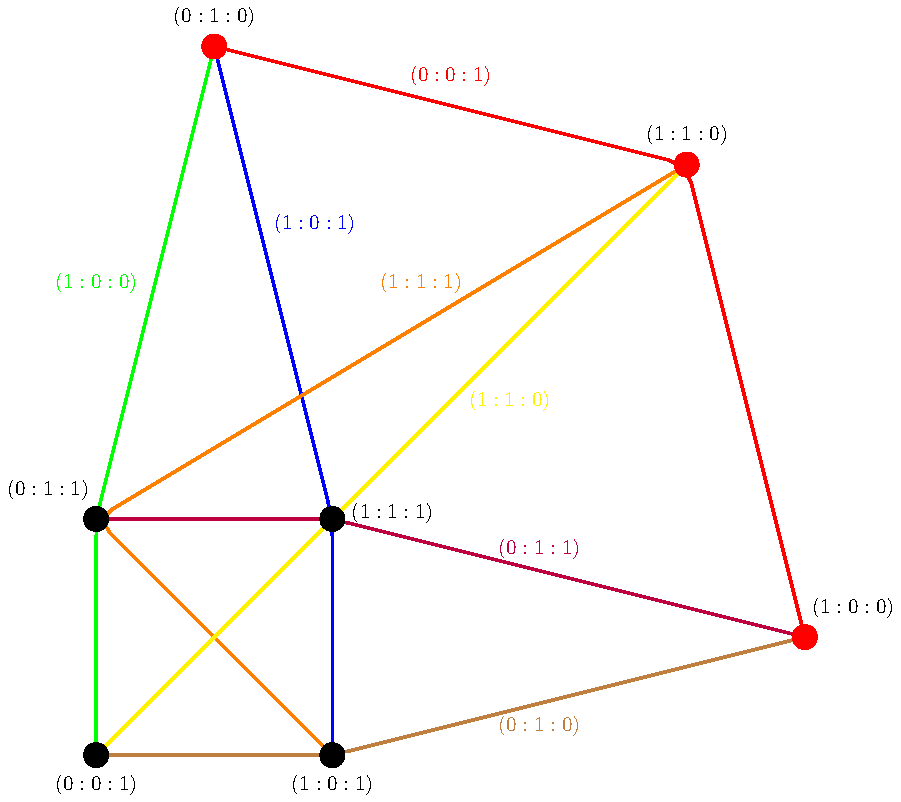
\includegraphics[height=7cm]{droitestikz.pdf}};
 \node[anchor=east] at (6,8) { \begin{tabular}{|c|c|c|}
  \hline
  + & \textbf{0} & \textbf{1} \\
  \hline
  \textbf{0} & 0 & 1 \\
  \hline
  \textbf{1} & 1 & 0 \\
  \hline
  \end{tabular}
 };
\node[anchor=east] at (6,6) {\begin{tabular}{|c|c|c|}
  \hline
  $\times$ & \textbf{0} & \textbf{1} \\
  \hline
  \textbf{0} & 0 & 0\\
  \hline
  \textbf{1} & 0 & 1\\
  \hline
  \end{tabular}
};
\end{tikzpicture}
\end{frame}

\begin{frame}
  {\Huge Le jeu du Dobble}
  \begin{center}
  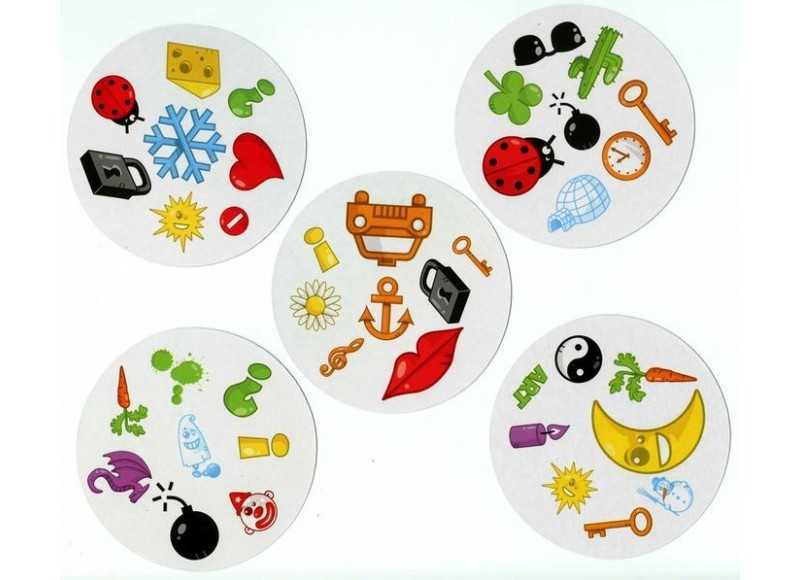
\includegraphics[width = 0.6\linewidth]{dobble.jpg}
  \end{center}
\end{frame}

\begin{frame}
  {\Huge Mon travail au LaBRI}
  \begin{center}
   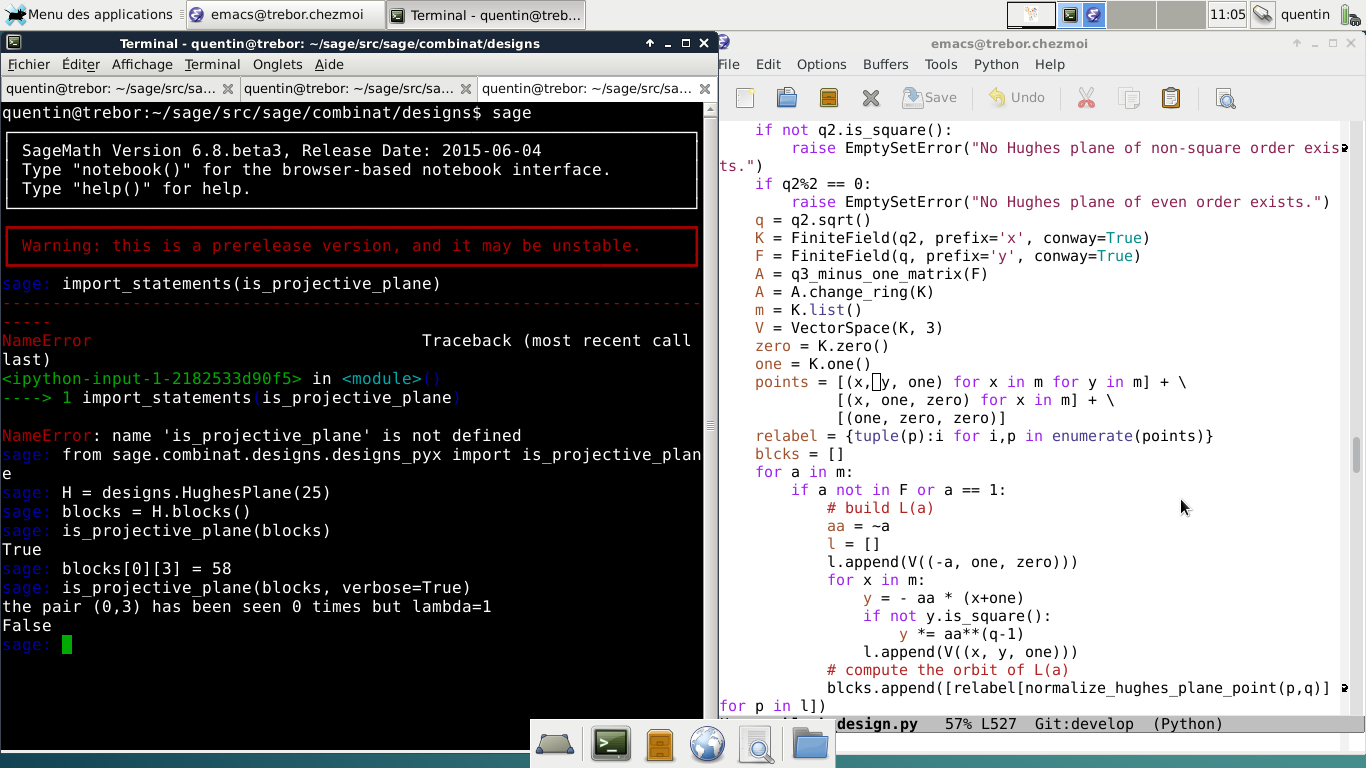
\includegraphics[height=5.5cm]{ecran.jpg}\bigskip\\

\href{trac.html}{
\includegraphics[height=0.5cm]{sagetrac.png}}
  \end{center}
  \end{frame}  

\end{document}
